%
% This is the source file for the paper ``rewriting open
% objects''. Here all categories A and X are topoi, as required for
% Open Objects to form a topos.
%

\documentclass{amsart}          

%
% PACKAGES
%

\usepackage{amsfonts}
\usepackage{amssymb}  
\usepackage{amsthm} 
\usepackage{amsmath} 
\usepackage{caption}
\usepackage[inline]{enumitem}
	\setlist{itemsep=0em, topsep=0em, parsep=0em}
	\setlist[enumerate]{label=(\alph*)}
\usepackage{doi}
\usepackage{etoolbox}
\usepackage{stmaryrd} 
\usepackage[dvipsnames]{xcolor}
	\definecolor{editcolour}{rgb}{0.7,0.5,0}
	\definecolor{hrefcolour}{rgb}{0,0,0.7}
\usepackage[]{hyperref}
	\hypersetup{colorlinks,linkcolor={hrefcolour},citecolor={hrefcolour},urlcolor={hrefcolour}}
\usepackage{graphicx}
	\graphicspath{ {img/} }
\usepackage{mathtools}
\usepackage[numbers]{natbib}
\usepackage{subcaption}
\usepackage{subfiles}
\usepackage{tikz}
	\usetikzlibrary{matrix,arrows,shapes,decorations.markings,decorations.pathreplacing}
\usepackage{todonotes}
\usepackage{url}

%
% COMMANDS
%

% mathbb
\newcommand{\RR}{\mathbb{R}}
\newcommand{\ZZ}{\mathbb{Z}}
\newcommand{\NN}{\mathbb{N}}
\newcommand{\QQ}{\mathbb{Q}}
\newcommand{\CC}{\mathbb{C}}
\newcommand{\DD}{\mathbb{D}}
\newcommand{\MM}{\mathbb{M}}
\newcommand{\LL}{\mathbb{L}}
\renewcommand{\epsilon}{\varepsilon}

% categories
\newcommand{\Set}{\cat{Set}}
\newcommand{\Graph}{\cat{Graph}}
\newcommand{\RGraph}{\cat{RGraph}}
\newcommand{\Top}{\cat{Top}}
\newcommand{\Cat}{\cat{Cat}}
\newcommand{\A}{\cat{A}}
\newcommand{\B}{\cat{B}}
\newcommand{\C}{\cat{C}}
\newcommand{\NonLinArrCat}{\cat{P}}
\newcommand{\LinArrCat}{\cat{C}}
\newcommand{\X}{\cat{X}}
\newcommand{\Y}{\cat{Y}}
\newcommand{\Z}{\cat{Z}}
\newcommand{\core}{\mathbf{core}}

% math formatting
\newcommand{\defn}[1]{\textbf{#1}}
\newcommand{\op}[1]{\operatorname{#1}}
\newcommand{\cat}[1]{\mathbf{#1}}
\newcommand{\dblcat}[1]{\mathbb{#1}}
\renewcommand{\t}[1]{\text{#1}}

% arrows
\newcommand{\from}{\colon}
\newcommand{\xto}[1]{\xrightarrow{#1}}
\newcommand{\xgets}[1]{\xleftarrow{#1}}
\newcommand{\tospan}{\xrightarrow{\mathit{sp}}}
\newcommand{\tocospan}{\xrightarrow{\mathit{csp}}}
\newcommand{\diagram}[1]{\raisebox{-0.5\height}{\includegraphics{#1}}}

% (co)span double/bi/1 categories
\newcommand{\Span}{\mathbf{Span}}
\newcommand{\MonicSpan}[1]{\mathbf{MonSpan}}
\newcommand{\SSpan}{\mathbb{S}\mathbf{p}}
\newcommand{\Cospan}{\mathbf{Cospan}}
\newcommand{\CCospan}{\mathbb{C}\mathbf{sp}}
\newcommand{\SpSp}[1]{\mathbf{Sp}(\mathbf{Sp}(#1))}
\newcommand{\SSpSp}[1]{\mathbb{S}\mathbf{p(\mathbf{Sp}(#1))}}
\newcommand{\CspCsp}[1]{\mathbf{Csp}(\mathbf{Csp}(#1))}
\newcommand{\CCspCsp}[1]{\mathbb{C}\mathbf{sp}(\mathbf{Csp}(#1))}
\newcommand{\MonSpCsp}[1]{\mathbf{MonicSp}(\mathbf{Csp}(#1))}
\newcommand{\MMonSpCsp}[1]{\mathbb{M}\mathbf{onicSp}(\mathbf{Csp}(#1))}
\newcommand{\EpCspSp}[1]{\mathbf{EpicCsp}(\mathbf{Csp}(#1))}
\newcommand{\EEpCspSp}[1]{\mathbb{E}\mathbf{picCsp}(\mathbf{Sp}(#1))}
\newcommand{\SpCsp}[1]{\mathbf{Sp}(\mathbf{Csp}(#1))}
\newcommand{\SSpCsp}[1]{\mathbb{S}\mathbf{p}(\mathbf{Csp}(#1))}
\newcommand{\FuncCsp}[1]{ #1 \t{-} \mathbf{Csp}}
\newcommand{\OpenOb}{\mathbf{Open} }
\newcommand{\Rewrite}{\mathbf{Rewrite} }
\newcommand{\RRewrite}{ \mathbb{R}\mathbf{ewrite} }
\newcommand{\MonRewrite}{ \mathbf{MonRewrite}}
\newcommand{\MMonRewrite}{ \mathbb{M}\mathbf{on}\mathbb{R}\mathbf{ewrite} }

% editting
\newcommand{\edit}[1]{\textcolor{editcolour}{(#1)}}

%
% MATH OPERATORS
%

\DeclareMathOperator{\Hom}{Hom}
\DeclareMathOperator{\id}{id}
\DeclareMathOperator{\ob}{Ob}
\DeclareMathOperator{\arr}{arr}
\DeclareMathOperator{\im}{im}
\DeclareMathOperator{\Aut}{Aut}
\DeclareMathOperator{\Bij}{Bij}
\DeclareMathOperator{\Sub}{Sub}
\DeclareMathOperator{\colim}{colim}

%
% ENVIRONMENTS & COUNTERS
%

\newenvironment{exposition}[1]{}{}

\newtheorem{theorem}{Theorem}[section]
\newtheorem{lemma}[theorem]{Lemma}
\newtheorem{proposition}[theorem]{Proposition}
\newtheorem{corollary}[theorem]{Corollary}

\theoremstyle{remark}
	\newtheorem{remark}[theorem]{Remark}
	\newtheorem{notation}[theorem]{Notation}

\theoremstyle{definition}
	\newtheorem{example}[theorem]{Example} 
	\newtheorem{definition}[theorem]{Definition}
          
% \setcounter{tocdepth}{1} % Sets depth for table of contents. 

%
% TIKZ TYPES
%
\tikzset{->-/.style={decoration={%
			markings,
			mark=at position .5 with {\arrow{>}}},postaction={decorate}}
}
\tikzset{->-pos/.style={decoration={%
			markings,
			mark=at position #1 with {\arrow{>}}},postaction={decorate}}
}
\tikzset{->-/.style={decoration={%
			markings,
			mark=at position .5 with {\arrow{>}}},postaction={decorate}}
}
\tikzset{->-pos/.style={decoration={%
			markings,
			mark=at position #1 with {\arrow{>}}},postaction={decorate}}
}

%
% INLINE DIAGRAMS
%
\newcommand{\rgraph}[2]{%
	$\begin{tikzpicture}
	\node (a) at (0,0) {$ #1 $};
	\node (b) at (1,0) {$ #2 $};
	\draw [->] (a.30) to (b.150);
	\draw [->] (a.-30) to (b.-150);
	\draw [->] (b) to (a);
	\end{tikzpicture}$
}
\newcommand{\graph}[2]{%
	$\begin{tikzpicture}
	\node (a) at (0,0) {$ #1 $};
	\node (b) at (1,0) {$ #2 $};
	\draw [->] (a.30) to (b.150);
	\draw [->] (a.-30) to (b.-150);
	\end{tikzpicture}$
}

\author{Daniel Cicala}
\title{Rewriting open objects}

% end preamble________________________
%_____________________________________
%_____________________________________
%_____________________________________
%_____________________________________
%_____________________________________
%_____________________________________

\begin{document}

\maketitle{} 

% end begin document__________________
%_____________________________________
%_____________________________________
%_____________________________________
%_____________________________________
%_____________________________________
%_____________________________________

\section{Introduction}
\label{sec:introduction}

The goal of this paper is to present a bicategorical framework in
which to study rewriting in open networks.

By an \emph{open network}, we mean a network together with a boundary.
To make this precise, we begin with a category of `input and output
types' $\cat{C}$ and another category of `networks' $ \cat{D} $.  To
equip a network, an object of $\cat{D}$, with a boundary, a pair of
objects from $\cat{C}$, we use an adjunction

\[ % adjoint diagram
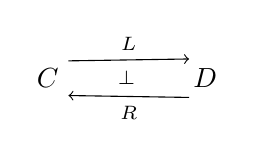
\begin{tikzpicture} 
  \node (C) at (0,0) {$ C $};
  \node (D) at (2,0) {$ D $};
  \node at (1,0) {\scriptsize $ \perp $};
  \draw [->] (C.40) to 
  node [above] {\scriptsize $ L $} (D.130);
  \draw [<-] (C.-40) to 
  node [below] {\scriptsize $ R $} (D.-130);
\end{tikzpicture}
\]

With this setup, we focus on three categories.  The first category,
denoted $ \Span_L $, has as objects, those from $ \cat{C} $, and as
arrows, cospans of the form
\[
Lc \to d \gets Lc'
\]
inside of $ \cat{D} $. 

The second category, denoted \edit{whatever it is}, has cospans
\[
Lc \to d \gets Lc'
\]
in $ \cat{ D } $ for objects and triples of arrows $ ( f , g , h ) $
such that y
\[ % diagram for L-open arrows
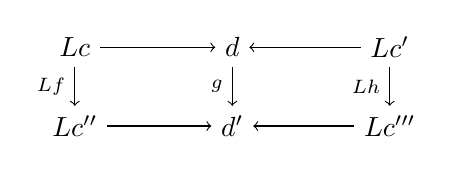
\begin{tikzpicture}
  \node (Lc) at (-2,1) {$ Lc $};
  \node (d) at (0,1) {$ d $};
  \node (Lc') at (2,1) {$ Lc' $};
  \node (Lc'') at (-2,0) {$ Lc'' $};
  \node (d') at (0,0) {$ d' $};
  \node (Lc''') at (2,0) {$ Lc''' $};
  \draw [->] (Lc) to (d);
  \draw [->] (Lc') to (d);
  \draw [->] (Lc'') to (d');
  \draw [->] (Lc''') to (d');
  \draw [->] (Lc) to node [left] {\scriptsize $ Lf $ } (Lc'');
  \draw [->] (d) to node [left] { \scriptsize $ g $ }(d');
  \draw [->] (Lc') to node [left] { \scriptsize $ Lh $ }(Lc''');
\end{tikzpicture}
\]
commutes.
We show that, when $ \cat{C} $ and
$ \cat{D} $ are topoi, then so is $ \edit{insrt} $.

The third category, denoted $ \edit{insert} $, again has cospans
\[
Lc \to d \gets Lc'
\]
in $ \cat{D} $ for objects and \emph{cubical spans of cospans}, that
is commuting diagrams
\[ % cubical span of cospans
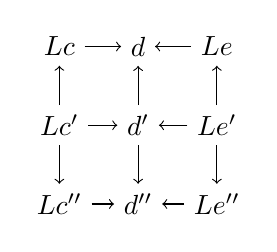
\begin{tikzpicture}
  \node (Lc) at (-1,1) {$ Lc $};
  \node (Lc') at (-1,0) {$ Lc' $};
  \node (Lc'') at (-1,-1) {$ Lc'' $};
  \node (d) at (0,1) {$ d $};
  \node (d') at (0,0) {$ d' $};
  \node (d'') at (0,-1) {$ d'' $};
  \node (Le) at (1,1) {$ Le $};
  \node (Le') at (1,0) {$ Le' $};
  \node (Le'') at (1,-1) {$ Le'' $};
  \draw [->] (Lc) to (d);
  \draw [->] (Le) to (d);
  \draw [->] (Lc') to (d');
  \draw [->] (Le') to (d');
  \draw [->] (Lc'') to (d'');
  \draw [->] (Le'') to (d'');
  \draw [->] (Lc') to (Lc);
  \draw [->] (Lc') to (Lc'');
  \draw [->] (d') to (d);
  \draw [->] (d') to (d'');
  \draw [->] (Le') to (Le);
  \draw [->] (Le') to (Le'');
\end{tikzpicture}
\]
for arrows.  

How do these three categories help us to model open networks?  To
answer this, we first make the observation that cospans of the form
\[
Lc \to d \gets Lc'
\]
have showed up in each of the above categories. We call such cospans
\emph{$L$-open objects}.  The term ``open'' indicates that we are
thinking of $d$ as an object that can `interact' with certain
elements. More concretely, we say that $ d $ has inputs $Lc$ and
outputs $ Lc' $ which allow $ d $ to be glued together with any other
$ L $-open object with outputs $ Lc $ or inputs $ Lc' $.  This would
give us a zig-zag which we turn into an $ L $-open object via pushout.
But this is exactly the composition in $ \edit{insert} $. Hence,
through their `openness' we can think of $ L $-open objects as arrows.
This is not the only perspective we take, however.

Through the categories $ LopenD $ and $ LrewriteD $, we can think of $
L $-open objects as, well, objects.  Certainly, the arrows of $ LopenD
$ are the best candidate for a morphism of $ L $-open objects.  We
show that $ LopenD $ is actually a topos.  Then, by work of Lack and
Sobocinski, we know that $ L $-open objects admit a nice (double
pushout) rewriting theory. The sort of rewriting theory we are
interested in, and that Lack and Sobocinski study, uses spans
\[
\ell \to k \gets r
\]
to say that the object $ \ell $ is rewritten to the object $ r $,
where $ k $ is some interface common to both $ \ell $ and $ r $.
Translating this to the topos $ LopenD $, we consider spans of $ L
$-open objects which are exactly the arrows for $ LrewriteD $.
Therefore, we think of $ LopenD $ as the category of $ L $-open
objects with their morphisms and $ LrewriteD $ as the category of $ L
$-open objects and their rewrite rules.

HERES A CHANGE

% end intro___________________________
%_____________________________________
%_____________________________________
%_____________________________________
%_____________________________________
%_____________________________________
%_____________________________________

\section{A motivating example}
\label{sec:motivating-example}

This section serves two functions. First, we discuss the example that motivates this paper.  Within our discussion, we take the opportunity to set both notation and language used in the sequel.  

When reading network theory literature written from the compositional perspective, one comes across the notion of an open graph. 
	\todo{cite}
The level of formality this definition is given varies between authors, but the core idea is that an \emph{open graph} is a $ \Set $-diagram $ E \rightrightarrows N $ together with a subset $ L \subseteq N$ equipped with a partition $ L = L_{ \t{in} } + L_{ \t{out} } $.
	\todo{insert diagram D1-open graph}
The conceit is that the subset of nodes $ L $ is a boundary that is accessible to other open graphs. Elements of $ L_{ \t{in} } $ and $ L_{ \t{out} } $ are thought of as inputs and outputs, respectively.  Given two open graphs $ (E \rightrightarrows N , L_{ \t{in} } + L_{ \t{out} }) $ and $ (E' \rightrightarrows N' , L'_{ \t{in} } + L'_{ \t{out} }) $, such that $ L_{ \t{out} } = L'_{ \t{in} } $, then we can construct the graph $ (E + E' \rightrightarrows (N + N') / L_{ \t{out} } = L'_{ \t{in} } ,  L_{ \t{in} } + L'_{ \t{out} } ) $.  For example,
	\todo{insert diagram D2-glueing open graphs}.
We casually add that by appropriately modifying the definition of a graph morphism, one can define a morphism of open graphs.

A primary motivation behind this construction is to model the process of connecting networks together.  Although, some networks contain additional information that cannot be conveyed by an open graph as described above.
	\todo{cite examples: circ, zx-calc, petri nets, etc}
To accommodate such demands, we generalize the notion of an open graph to that of an \emph{open object} and develop some basic theory for open objects.  

One feature that distinguishes this work from other related work is
our preference for reflexive graphs over directed graphs.  Before
mentioning our reasons, let us clarify exactly what we mean by these
two sorts of graphs. Denote by $ \rgraph{\bullet}{\bullet} $ the
category with two objects $ [0] $ and $ [1] $ with two arrows
$ s,t \from [1] \to [0] $ and an arrow $ r \from [0] \to [1] $ that is
a section to both $ s $ and $ t $.  Throughout this text, the category
of reflexive graphs is
$ \RGraph \coloneqq [ \rgraph{\bullet}{\bullet} , \Set] $ and the
category of directed graphs is
$ \Graph \coloneqq [ \graph{\bullet}{\bullet} , \Set ] $.  The reasons
for working with reflexive graphs are myriad.  For one, elements
$ 1 \to \Gamma $ of a graph $ \Gamma $ are not just nodes, but nodes
with a loop attached.  It follows that the underlying nodes functor
$ \RGraph \to \Set $ is representable by the terminal graph. This is
not the case for the underlying nodes functor of type
$ \Graph \to \Set $.  Also, the objects of $ \RGraph $ are truncated
simplicial sets. The advantage of this goes, perhaps, beyond the scope
of this paper. Suffice to say, when working with graph relations,
particularly those homotopical in nature, we desire a well-known model
structure to work with.  Having said this, let it be known that from
this point, any reference to a ``graph'' will mean a ``reflexive
graph'' unless specified otherwise. This includes cases when we modify
``graph'' with an adjective. For instance, by ``open graph'' we
actually mean ``open reflexive graph''.

Because open graphs are the archetypal example of an open object, it behooves us to formalize that which we have so far glossed over. 

\begin{definition} \label{df:OpenGraph}
  Let $ L \from \Set \to \RGraph $ be
  the discrete graph functor.  An \textbf{open graph} is a cospan of
  the form $ L x \to \gamma \gets L y $.
\end{definition}

In this definition, there is a graph $ \gamma $ with input nodes $ Lx $ and output nodes $ Ly $.  The functor $ L $ allows us to simultaneously treat graph boundaries $ Lx + Ly $ as both separate from and part of the graph.  

Immediately emerging are two perspectives on open graphs, both alluded
to above. The first we call \emph{the structured cospan
  perspective}. From this point of view, we want to be able to glue
together suitable open graphs to form new open graphs. This leads one
to consider a category with sets as objects as with open graphs $ Lx
\to \gamma \gets Ly $ as arrows of type $ x \to y $.  Composition uses
pushouts as is typical in cospan categories.  Heuristically, pushing
out can be thought of as a ``categorical gluing''.  \todo{ref diagram
  abv?}  The second perspective is called the \emph{open object
  perspective}.  Here, we treat open graphs as mathematical objects
deserving of their own morphisms.  Indeed, a morphism
\[
(L x \to \gamma \gets L y) \to ( L x' \to \gamma' \gets L y' )
\]
of open graphs is a a commuting diagram
\[
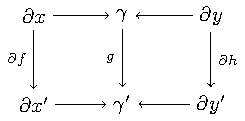
\includegraphics{diag_open-graph-morph_reopn}
\]
This leads to another category where open graphs are objects, as opposed to arrows.  

Having two categories featuring open graphs---one as arrows, the other
as objects---one can construct a double category containing all of
this structure.  This double category is defined to have sets as
0-cells, set functions as vertical 1-cells, open graphs as horizontal
1-cells and morphisms of open graphs as 2-cells.  The composition
functor of this double category takes advantage of the fact that open
graphs are also arrows of a category.  \todo{include D4 composition
  diagram} Later, we prove that this actually forms a double category.

In fact, we do this in Section BLAH. 
	\todo{input appropriate section}
In the following section, we generalize open graphs to `open objects' and construct a pair of categories, one with open objects as arrows and the other with open objects as objects.  

% end section: motivating example____________________________
%____________________________________________________________
%____________________________________________________________
%____________________________________________________________
%____________________________________________________________
%____________________________________________________________

\section{Open objects and structured cospans}
\label{sec:open-objects}

For good, we set a cocartesian geometric morphism between (elementary)
topoi
  \[
    \diagram{diag_oo_geometric-morphism}
  \]
Although many of the definitions and theorems work with slightly
greater levels of generality, we content ourselves with this
restriction. For one, it is really not much of a constraint at
all. Second, it greatly simplifies the statements of various
definitions and theorems.
  
Additionally, we will write a cospan
\[
    x \to y \gets z
\]
as a triple \( (x,y,z) \) when our work does not require us to name
the arrows.
  
We develop a theory of ``open objects'' with the intention of applying
it to study open networks.  These are not defined precisely at this
point, but suffice to say that a typical example is a sort of graph
with additional information attached to its nodes and edges.  The
motivating example for us is the category of open graphs.  There are
various definitions of open graphs in the literature \emph{(cite)},
but we define in a way we believe is more susceptible to
generalization.  The motivating example is to start with the
adjunction $ L \dashv R \from \Set \to \RGraph $ between sets and
reflexive graphs where $ L $ gives the discrete graph on the nodes of
a set and $ R $ returns the points of a graph.  An \defn{open graph}
is a cospan $ ( La , g , Lb ) $.  Think of this data as a graph $ g $
with inputs $ La $ and outputs $ Lb $.  The reason for choosing
reflexive graphs instead of directed graphs is primarily aesthetic.
For one, we like to think of the nodes of a graph as \emph{points}, a
notion formalized in categories by arrows from the terminal object.
It is therefore morally desirable for a so-called `discrete graph'
functor to be represented by the terminal set. It is also structurally
desirable as well, since working with reflexive graphs instead of
directed graphs provides a left exact `discrete graph' functor.
 
Our first task is to provide an abstract framework in which this
example organically fits.

\begin{definition} \label{df:struct-cospan}
  Denote by \( \Cospan_L \) the category with objects from \( \A \)
  and whose arrows of type \( a \to b \) are cospans \( La \to x \gets
  Lb \) in \( \X \). We call these arrows \defn{ \( L \) -structured
    cospans}.
\end{definition}

Our interest lies primarily in arrows from \( \Cospan L \) .  We will
use such cospans to encode open networks by tying the cospan feet as
choosing the inputs and outputs of a network $ x $. At times, it is
helpful for us to view these as arrows in a category, but it will
often be helpful to view them as objects as well.  However, in
behooves us to work in maximum generality. Therefore, we do not
immediately bind ourselves to working with networks even though they
are the chief motivation.  Instead, we refer to $ \Cospan_L $-arrows
as \defn{$ L $-open objects}.  The ``\( L \)-open'' indicates that
objects in $ \X $ can interact with one another via an interface
determined by $ L $.  The precise interaction is described by
composing cospans in the usual manner.

\begin{definition} \label{df:open-objects}
  Denote by $ \OpenOb $ the category whose objects are \( L \)
  -structured cospans and arrows are commuting diagrams
  % \[
  %   \diagram{diag_openob_openob-arrow}.
  % \]
  
  Even though \( \OpenOb \) depends on \( L \), we can safely reject
  \( L \) from our notation because we have no cause to consider open
  objects with respect to a differently named functor.

  \edit{ Is OpenOb functorial? If so, we'll need to include the
    functor name in the notation, at least until we prove it's functorial.}
\end{definition}

\begin{remark} \label{thm:open-obj-ptwise-limits}
  Limits and colimits in \( \OpenOb \) are computed pointwise. This
  follows from the fact that \( \OpenOb \) is a subcategory of \(
  \left[ \bullet \to \bullet \gets \bullet \right] , \X \).   
\end{remark}

Having both $ \Cospan_L $ and $ \OpenOb $ around allow us to view open
objects with two different perspectives.  The perspective \( \Cospan_L
\) provides a compositional one. And \( \OpenOb \) sees an open object
as a space. The latter perspective is substantiated by the following
theorem.

% thmA
\begin{theorem} \label{thm:OpenObTopos}
  Then $ \OpenOb $ is a topos.
\end{theorem}

\edit{Is this function functorial?  What are geometric morphisms
  between topoi of the form $ \OpenOb{\partial} $?  Geometric natural
  transformations?  Does this correspond to natural transformation in
  category of topoi with geometric morphisms?}

Because $ \OpenOb $ is a topos, it admits a double
pushout rewriting system, the topic of our next section.

% end open obs & structured cospans________________________
%__________________________________________________________
%__________________________________________________________
%__________________________________________________________
%__________________________________________________________
%__________________________________________________________
%__________________________________________________________

\section{Double pushout rewriting}
\label{sec:double-push-rewr}
  
\begin{definition} \label{df:dpo_adhesive-category} 
  A category with pullbacks is \defn{adhesive} if pushouts along
  monics exist and are \emph{Van Kampen}.
\end{definition} 

% thmB
\begin{theorem} \label{thm:dpo_topoi-adhesive} 
  Topoi are adhesive.
\end{theorem}

\begin{corollary} \label{thm:dpo_category-StrCsp-adhsv}
  The category $ \OpenOb $ is adhesive.
\end{corollary}

\begin{remark}
  Moving forward, we only work with topoi with the understanding that
  they are adhesive, hence suitable hosting double pushout rewriting.
  However, much of what we uncover is generalizable to the broader
  world of adhesive categories.
\end{remark}

\begin{definition} \label{df:dpo_rewrite-rule} 
  For $ \cat{T} $ a topos, a \defn{$ \cat{T} $-rewrite rule}
  (often called a production) is a span $ a \gets b \to c $ inside
  $ \cat{T} $.  When both legs of the span are monic, we say the rewrite
  rule is \defn{linear}.
\end{definition}	

\begin{definition} \label{df_dpo_pushout-complement} 
  Given composable arrows $ a \to b \to y $ we say that an arrow
  $ a \to x $ is a \defn{pushout complement} if it fits into a pushout
  diagram
  \[
    \diagram{diag_rw_pushout-comp}
  \]
  Pushout complements are unique up to isomorphism when the arrow \( a
  to b \) is monic.

  \edit{cite adhesive paper}
\end{definition}

\begin{definition} \label{df:dpo_derived-rewrite-rule} 
  Fix a \( \cat{T} \) -rewrite rule \( a \gets b \to c \) and a
  $ \cat{T} $-arrow $ a \to x $ such that $ b \to a \to x $ has a 
  pushout complement. A \defn{derived (linear) rewrite rule} is the
  bottom row of the induced double pushout diagram 
  \[ 
    \diagram{diag_rw_derived-rule}
  \]
\end{definition}

\begin{definition} \label{df:dpo_grammar}
  A \defn{ grammar } consists of a topos \( \cat{T} \) and a set of
  \( \cat{T} \) -rewrite rules. The \textbf{language}
  \( \mathcal{L} ( \Gamma ) \) for a grammar \( \Gamma \) is a set
  consisting of all rewrite rules derived from \( \Gamma \).
\end{definition}

\begin{remark}
  Note that a language is a set of arrows from \( \Span ( \cat{T}
  \). This observation is put to use later on.   
\end{remark}

\begin{remark}
  The notion of `adhesive categories' does not show up in the
  definition of grammar or language.  So, of course, one can talk
  about grammars in \emph{any} category.  However, working within an
  adhesvie category ensures we have nice properties.

  \edit{ what nice properties? } 
\end{remark}

% end dpo rewriting_____________________________________________
%_______________________________________________________________
%_______________________________________________________________
%_______________________________________________________________
%_______________________________________________________________
%_______________________________________________________________
%_______________________________________________________________

\section{Non-linear rewriting}
\label{sec:non-linear-rewriting}

\edit{Current goal : define double category non-linear
  rewriting. subgoals: define object // arrow categories }

Throughout this section, we refer to diagrams with the form
\begin{equation}
  \label{eq:nlr-2cell-form}
  \diagram{diag_nlr_dbl-rewrite-2cell}
\end{equation}
where $ \alpha $, $ \alpha' $, $ \beta $, and $ \beta' $ are isomorphisms in $ \A $

%%%%%%%%%%%%%%%%% *SUBSECTION*
%%%%%%%%%%%%%%%%%   NON-LINEAR REWRITES

\subsection{A double category for non-linear rewriting}
\label{sec:dbl-cat-nonlinr-rewr}

\begin{lemma} \label{thm_dbl-rewr-obcat}
  There is a symmetric monoidal category
  $ ( \core (\Span (\A)) , \otimes , I , \tau ) $ defined as follows:

  \begin{itemize}
    \item $ \core (\Span (\A)) $ is the subcategory of $ \Span (\A) $
      consisting of all objects and whose arrows have invertible legs,
    \item $ \otimes $ is the pointwise application of $ + $,
    \item $ I $ is the span consisting of identities on $ 0_{\A} $,
    \item $ \tau $ is the pointwise application of $ \tau_{\A} $.
  \end{itemize}
\end{lemma}

\begin{proof}
  The only non-trivial thing to check is that the interchange law
  holds between tensor and composition.  That is, given two pairs of
  composable spans $ a \gets b \to c $, $ c \gets d \to e $ and
  $ a' \gets b' \to c' $, $ c' \gets d' \to e' $, we show that the
  span obtained by tensoring before composing
  \[
    a + a' \gets (b + b') \times_{c + c'} (d + d') \to e + e'
  \]
  is equal to the span obtained by composing before tensoring
  \[
    a + a' \gets (b \times_{c} d) + (b' \times_{c'} d') \to e + e'.
  \]
  In this context, equality means isomorphic as spans. But this
  follows from local cartesian closedness, because pullback functors
  are all left adjoints.
\end{proof}

\begin{lemma} \label{thm:dlb-rewr-arrcat}
  There is a symmetric monoidal preorder
  $ ( \NonLinArrCat , \otimes , I , \tau ) $ defined as follows:
  
  \begin{itemize}
  \item $ \NonLinArrCat $ has $ L $-open objects and an arrow
    $ ( La , x , La') \leq ( Lc , x , Lc') $ whenever
    there is commuting diagram of form \eqref{eq:nlr-2cell-form},
   \item $ \otimes $ is given by
       \[
         \diagram{diag_nlr_dbl-rewrite-tensor}
       \]
   \item $ I $ is given by a pair of identities on $ L0_{\A} $
   \item $ \tau $ is given by
     \[
	\diagram{diag_nlr_dbl-rewrite-braiding}
     \]
   \end{itemize}
\end{lemma}
  
\begin{proof}
  The only non-trivial thing to check is that the tensor and
  composition satisfy interchange. That is, given two pairs of
  composable arrows
  \[
    \diagram{diag_nlr_preorder-interchange}
  \]
  we want to show that the resulting arrow obtained by tensoring
  before composing
  \[
    \diagram{diag_nlr_preorder-tensor-compose}
  \]
  is equal to the arrow obtained by composing before
  \[
    \diagram{diag_nlr_preorder-compose-tensor}
  \]
  These arrows are parallel, hence equal by definition.
\end{proof}

\begin{lemma} \label{thm:preord-symm}
  The preorder $ \NonLinArrCat $ is symmetric.
\end{lemma}
 
\begin{proof}
  Any arrow $ ( La , x , La' ) \leq ( Lc , z , Lc' ) $ in
  $ \NonLinArrCat $ gives an arrow
  $ ( Lc , z , Lc' ) \leq ( La , x , La' ) $ by taking the
  dual span of $ L $-structured cospans.
\end{proof}

\begin{comment} 
  There is a symmetric monoidal double category $ \RRewrite_{L} $ with
  $ \A $-objects as 0-cells, spans in $ \A $ with invertible legs as
  vertical 1-cells, $ L $-structured cospans \edit{open objects?}  as
  horizontal 1-cells, and a unique 2-cell if there exists a commuting
  diagram in $ \X $ of form \eqref{eq:nlr-2cell-form}
\end{comment}

% thmC
\begin{theorem} \label{thm:dbl-rewr-smc}
  There is a symmetric monoidal double category
  $ ( \RRewrite_{L} , \otimes , I, \tau ) $ consisting of the
  following data
  
  \begin{enumerate}
    \item object category $ \RR_0 \coloneqq \core ( \Span (\A) ) $;
    \item arrow category $ \RR_1 \coloneqq \NonLinArrCat $;
    \item unit functor $ U \from \RR_0 \to \RR_1 $ defined by
      \[
        \diagram{diag_nlr_dbl-rewrite-unit-functor}
      \]
    \item source and target functors $ S , T \from \RR_1 \to \RR_0 $
      respectively defined by
      \[
        \diagram{diag_nlr_dbl-rewrite-source-functor}
        \quad \text{and} \quad
        \diagram{diag_nlr_dbl-rewrite-target-functor}
      \]
    \item composition functor
      $ \odot \from \RR_1 \times_{\RR_0} \RR_1 \to \RR_1 $ defined by
      \[
        \diagram{diag_nlr_dbl-rewrite-composition-functor}
      \]
      which uses pushouts in $ \X $ and their universal properties
    \item The tensor $ \otimes $ is given by
      \[
        \diagram{diag_nlr_dbl-rewrite-tensor}
      \]
    \item a monoidal unit $ I $ defined by
      \[
        I \coloneqq ( L I_{\A} \to L I_{\A} \gets L I_{\A} )
      \]
   \item and braiding $ \tau $ defined by
     \[
       \diagram{diag_nlr_dbl-rewrite-braiding}
     \]
   \end{enumerate}
\end{theorem}

\begin{proof}
  Composition is functorial because $ \RR_1 $ is a preorder. It is
  straightforward to check that $ S;U = \id = T;U$ and that applying
  $ S $ and $ T $ to
  \[
    \diagram{diag_nlr_dbl-rewrite-deconstructed-composite}
  \]
  respectively returns \( ( La , Lb , Lc ) \) and \( ( La'' , Lb'' ,
  Lc'' ) \).
  
  The associator, plus left and right unitors are defined using
  universal properties. Therefore, $ \RRewrite_L $ is a double
  category.
	
  We now show that it is symmetric monoidal.  For this, we follow
  Shulman's unpacking of Definition \edit{blah}.  \todo{citation}
  Lemmas \ref{lem_IRewrite-obcat} and \ref{lem_IRewrite-arcat} show
  that our object and arrow categories are symmetric monoidal.  We
  have that $ U ( 0 ) $ is the pair of identities on $ L 0 $ and that
  the source $ S $ and target $ T $ functors are strict monoidal by
  construction.
	
  Next, given two pairs of composable vertical arrows
  \[
    \diagram{diag_nlr_dbl-rewrite-interchange}
  \]
  we construct an invertible 2-cell (denoted $ \mathfrak{X} $ by
  Shulman) of form
  \begin{equation} \label{eq:dlb-rewr-intchng-2cell}
    \diagram{diag_nlr_dbl-rewrite-interchange-2cell}
  \end{equation}
  The cospans along the top and bottom of
  \eqref{eq:dlb-rewr-intchng-2cell} follow from, respectively,
  tensoring before composition and composing before tensoring. The map
  $ \theta $ is constructed below. Denote the monoidal structure map
  by $ s $, a canonical inclusion by $ \iota $, and a canonical
  quotient by $ q $.  The cospan along the top of
  \eqref{eq:dlb-rewr-intchng-2cell} has arrows from the diagram
  \[
    \diagram{diag_nlr_dbl-rewrite-tensor-compose}
  \]
  and the cospan along the bottom has arrows from the diagram
  \[
    \diagram{diag_nlr_dbl-rewrite-compose-tensor}
  \]
  The arrow $ \theta $ in \eqref{eq:dlb-rewr-intchng-2cell} exists
  because of the universal property of a pushout.  The diagram
  \[
    \diagram{diag_nlr_dbl-rewrite-pushout-competetor}
  \]
  commutes because the equations $ g ; \iota ; q = h ; \iota ; q $ and
  $ g' ; \iota ; q = h' ; \iota ; q $ hold.  Indeed, these equations
  are exactly those from the pushout squares of $ w +_{Lb} x $ and
  $ y +_{Lb'} z $.  It follows that $ \theta $ fits into diagram
  \eqref{diag_IRewrite-interchange-2cell-form}. Because $ \RR_1 $ is a
  symmetric preorder (Lemma \ref{lem_IRewrite-arcat-isSym}), the
  2-cell \eqref{diag_IRewrite-interchange-2cell-form} is invertible as
  required.
	
  Next, for objects $ a $ and $ b $, we need an invertible 2-cell
  (denoted $ \mathfrak{u} $ by Shulman) $ U(a + b) \to Ua + Ub
  $. Again, to Lemma \ref{thm:preord-symm} ensures that all 2-cells
  are invertible.  Therefore, the 2-cell
  \[
    \diagram{diag_nlr_dbl-rewrite-unit-functor-2cell}
  \]
  provides $ \mathfrak{u} $
	
  It remains to check that various coherence diagrams commute.  Each
  coherence diagram lives in the arrow category $ \RR_1 $ which is a
  preorder, so commutes automatically.
\end{proof}

% thmD
\begin{theorem} \label{thm:dbl-rewr-fibrant}
  The double category $ \RRewrite_L $ is fibrant.
\end{theorem}

\begin{proof}
  A companion for the vertical 1-cell $ a \xto{f} b \xgets{g} c $
  consists of the horizontal 1-cell
  $ La \xto{Lf^{-1}} Lb \xgets{Lg^{-1}} Lc $ together with the 2-cells
  \[
    \diagram{diag_nlr_dbl-rewrite-companion1}
    \quad \text{and} \quad
    \diagram{diag_nlr_dbl-rewrite-companion2}
  \]
  The equations hold because $ \RRewrite_L $ is locally posetal.
	
  A conjoint for the vertical 1-cell $ a \xto{f} b \xgets{g} c $
  consists of opposite horizontal 1-cell
  $ Lc \xto{Lg^{-1}} Lb \xgets{Lf^{-1}} La $ together with the same
  2-cells as the companion.  The equations hold because
  $ \RRewrite_L $ is locally posetal.
\end{proof}	

%%%%%%%%%%%%%%%%%%%% *SUBSECTION*
%%%%%%%%%%%%%%%%%%%% BICATEGORY FOR REWRITES

\subsection{A bicategory for non-linear rewrites}
\label{sec:bicat-nonlinr-rewr}

\begin{corollary} \label{thm:bicat-rewr-smc}
  The horizontal edge bicategory
  $ \Rewrite_{L} \coloneqq \mathcal{H} \left( \RRewrite_{L} \right) $
  in the sense of Shulman is symmetric monoidal.
\end{corollary}

\begin{proof}
  This follows from Theorem 5.1 in \edit{shulman cite} 
\end{proof} 

\begin{lemma} \label{thm:bicat-rewr-arrows-dual}
  Every 1-arrow of $ \Rewrite $ is a left and right adjoint.
\end{lemma}

\begin{proof}
  It is straightforward to check that $ ( La , x , Lb ) $ is both the
  left and right adjoint of $ ( Lb , x , La ) $.
\end{proof}

\begin{definition} \label{def:bicat-rels}
\edit{cite carb \& walts}
  Let $ \cat{B} $ be a bicategory whose hom-categories are posets. A
  \defn{Cartesian structure} on $ \cat{B} $ consists of a tensor
  product $ \otimes $ on $ \cat{B} $ and a cocommutative comonoid
  structure $ (\delta_x , \epsilon_x , \sigma_x ) $ on every object
  $ x $ in $ \cat{B} $.  In addition, this data satisfies two
  axioms. First, every 1-arrow $ f \from x \to y $ is a lax comonoid
  homomorphism, that is there are 2-arrows
  $ \delta_y f \Rightarrow (f \otimes f) \delta_x $ and
  $ \eta_y f \Rightarrow \eta_x $. Second, comultiplication and counit
  have right adjoints $ \delta^\ast_x $, $ \epsilon^\ast_x $. A
  Cartesian bicategory is said to be a \defn{bicategory of relations}
  if every object is a Frobenius object.
\end{definition}

% thmE
\begin{theorem} \label{thm:bicat-rewr-bicat-rel}
   The bicategory $ \Rewrite_{L} $ is a bicategory of relations in the
   sense of Carboni and Walters.
\end{theorem}

\begin{proof}
  We start by observing that $ \RRewrite $ is locally posetal because
  parallel 2-arrows are identified. The tensor product is provided in
  \ref{thm:bicat-rewr-smc}. We now show, in order, that each object
  has a cocommutative comonoid structure whose adjoints give a
  commutative monoid structure.  These are compatible via the
  Frobenius equation. Finally, every 1-arrow is a lax comonoid
  homomorphism.
	
  Given an object $ a $ in $ \RRewrite $, we use the folding map
  $ \Delta_{a} \from a + a \to a $ in $ \A $ to define
  comultiplication $ \delta_a \from a \to a + a $ as the cospan
  \[
    \delta_a \from La \to La \xgets{L\delta_a} L(a + a)
  \]
  and use the initial map to define the counit
  $ \epsilon_a \from a \to 0_a $ as the cospan
  \( (La \to La \gets L0_a) \).
  
  The associativity and unity 2-arrows appear canonically, as does
  cocommutativity.
	
  From that cocommutative comonoid structure, we obtain the
  commutative monoid structure by taking adjoints of all the 1-arrows
  (see \ref{thm:bicat-rewr-arrows-dual}).
	
  The Frobenius equations are witnessed by the commuting diagram
  \[
    \diagram{diag_nlr_bi-rewrite-frobenius}
  \]
  populated with arrows $ L \delta_a $.
	
  Finally, we need to check that any 1-arrow
  $ La \xto{f} x \xgets{g} Lb $ is a lax comonoid homomorphism. The
  lax comultiplication structure map comes from the commutating
  diagram
  \[
    \diagram{diag_nlr_bi-rewrite-lax-comul}
  \]
  made with $ f $, $ g $, the monoidal structure map
  $ s \from L(b+b) \to Lb+Lb $ and canonical arrows. The lax unit
  structure map comes from the commuting diagram
  \[
    \diagram{diag_nlr_bi-rewrite-lax-counit} \qedhere
  \]
\end{proof}

\begin{corollary} \label{thm:bit-rewr-comp-closed}
  The bicategory $ \Rewrite_L$ is compact closed.
\end{corollary}

\begin{corollary} \label{thm:bicat-rewr-freyds-modular}
  Freyd's modular law is satisfied:
  $ f (g \cap h) \Leftarrow h ( g^\circ \cap s ) r $.

  \edit{is$ ^\circ $ taking $ a \to b \gets c $ to
    $ c \to b\gets a $?}
\end{corollary} 

\begin{corollary} \label{thm:bicat-rewr-function-compl}
  Is it functionally complete? i.e. for each arrow
  $ r \from x \to I $, there is a map $ i \from x_r \to x $ such that
  $ i^\circ i = 1 $ and $ t i^\circ = r $, where $ t $ is a canonical
  map $ x_r \to I $. If so, then the subcategory of $ \Rewrite $ of
  maps (arrows with a right adjoint) is regular.
\end{corollary}

%%%%%%%%%%%%%%%%%%%%%% *SUBSECTION*
%%%%%%%%%%%%%%%%%%%%%%   NON-LINEAR REWRITES

\subsection{Double categories from non-linear grammars}
\label{sec:dblcats-nonlinr-gramrs}

\edit{ the below material on grammars was copied directly from the
  linear case and needs to be non-linearized. }

% thmF
\begin{lemma} \label{thm:lr_open-objects-language}
  Fix a grammar $ \Gamma $ of non-linear rewrite rules from the topos
  $ \OpenOb $. Then each element of the language
  $ \mathcal{L}(\Gamma) $ represents an arrow in \( \NonLinArrCat \) from
  \ref{thm:dlb-rewr-arrcat}. These arrows generate a symmetric
  monoidal sub-category of \( \NonLinArrCat \) which we denote by
  \( \NonLinArrCat_\Gamma \).

  \edit{ this can probably be worded and denoted better }
\end{lemma}

\edit{ does this need to be unpacked? }
  
\begin{definition} \label{df:gramr-gen-dbl-cat}
  Suppose each element from a grammar $ \Gamma $ in $ \OpenOb $ has
  form \eqref{eq:nlr-2cell-form}.  Denote by $ \LL ( \Gamma ) $ the
  symmetric monoidal double subcategory of $ \MMonRewrite_{L} $ whose
  object category is \( \core ( \Span ( \A ) ) \) and arrow category
  is \( \NonLinArrCat_\Gamma \).
\end{definition}

\edit{ how does the language of a grammar related to the double category? } 

% thmG
\begin{theorem}
  For any a pair of structured cospans \( (La,x,Lb) \) and
  \( (La',x',Lb' \) in a language \( \mathcal{L} (\Gamma) \), there
  are corresponding horizontal 1-cells in \( \LL (\Gamma) \). Then
  \( (La,x,Lb) \) can be written into \( (La',x',Lb') \) in
  \( \mathcal{L} (\Gamma) \) if and only if there is a 2-cell between
  the corresponding horizontal 1-cells in \( \LL (\Gamma) \).
\end{theorem}

% end non-linear rewriting__________________________________
%___________________________________________________________
%___________________________________________________________
%___________________________________________________________
%___________________________________________________________
%___________________________________________________________
%___________________________________________________________

\section{Linear rewriting}
\label{sec:linear-rewriting}

\todo{X shd b topos for intrchng}
\todo{remind linear meaning}

Throughout this section, we will refer to diagrams of the form
\begin{equation}
  \label{eq:ln-2cell-form}
  \diagram{diag_lr_dbl-mon-rewrite-2cell}
\end{equation}
where $ \alpha $, $ \alpha' $, $ \beta $, and $ \beta' $ are
invertible. The arrows marked ``$ \rightarrowtail $'' are monic.

%%%%%%%%%%%%%%%% *SUBSECTION*
%%%%%%%%%%%%%%%%   DOUBLE CATEGORY FOR LINEAR REWRITING

\subsection{A double category for linear rewriting}
\label{sec:dble-cat-linr-rewr}

\begin{definition} \label{def:mon-rewrite-obcat}
  Consider, again, a cocartesian category with pullbacks
  $ (\A , + , 0_{\A} , \tau_\A ) $
  that is locally cartesian closed and a monoidal category
  $ ( \core ( \Span ( \A )) , \otimes , I , \tau )$
  as in Lemma \ref{lem_IRewrite-obcat}.
\end{definition}

\begin{lemma} \label{thm:mon-rewrite-arrcat}
  There is a symmetric monoidal category
  $ ( \C , \otimes , I , \tau ) $ defined as follows:
  \begin{itemize}
   \item $ \C $ has $ L $-structured cospans \edit{open objects?}
          for objects and isomorphism classes of spans open objects of
          form \eqref{eq:ln-2cell-form}
   \item $ \otimes $ is given by
         \[
            \diagram{diag_lr_dbl-rewrite-tensor}
         \]
   \item $ I $ is given by a pair of identities on $ L0_A $
   \item $ \tau $ is given by
        \begin{center}
          \diagram{diag_lr_dbl-rewrite-braiding}
        \end{center}
   \end{itemize}
\end{lemma}

\begin{proof}
  Composition preserves monics because pullbacks do. Tensoring
  preserves monics because pushouts in adhesive categories preserve
  monics. Interchange holds between tensor and composition because
  pullback functors are left adjoints, thus preserve pushout. The
  remainder of the proof is a routine checking of axioms which we
  leave to the reader.
\end{proof}

\begin{lemma} 
  Denote by $ \MMonRewrite_{L} $ the double category with
  $ \A $-objects as 0-cells, spans in $ \A $ with invertible legs as
  vertical 1-cells, $ L $-structured cospans as horizontal 1-cells,
  and commuting diagrams in $ \X $ of form \eqref{eq:ln-2cell-form}
  \begin{itemize}
\item $ \otimes $ is given by
         \[
            \diagram{diag_lr_dbl-rewrite-tensor}
         \]
   \item $ I $ is given by a pair of identities on $ L0_A $
   \item $ \tau $ is given by
        \begin{center}
          \diagram{diag_lr_dbl-rewrite-braiding}
        \end{center}
   \end{itemize}
\end{lemma}

\begin{proof}
  Composition preserves monics because pullbacks do. Tensoring
  preserves monics because pushouts in adhesive categories preserve
  monics. Interchange holds between tensor and composition because
  pullback functors are left adjoints, thus preserve pushout. The
  remainder of the proof is a routine checking of axioms which we
  leave to the reader.
\end{proof}

\begin{lemma} \label{thm:dbl-mon-rewr-smc} 
  There is a symmetric monoidal double category
  $ (\MMonRewrite_{L} , \otimes , I , \tau) $. The double category
  $ \MMonRewrite_{L} $ consists of the object category
  $ \MM_0 \coloneqq \core (\Span (\A)) $; arrow category
  $ \MM_1 \coloneqq \C $; unit functor $ U \from \MM_0 \to \MM_1 $
  defined by
  \[
    \diagram{diag_lr_dbl-mon-rewrite-unit-functor}
  \]
  source and target functors $ S , T \from \MM_1 \to \MM_0 $
  respectively defined by
  \[
    \diagram{diag_lr_dbl-mon-rewrite-source-functor}
    \quad \text{and} \quad
    \diagram{diag_lr_dbl-mon-rewrite-target-functor}
  \]
  and composition functor
  $ \odot \from \MM_1 \times_{\MM_0} \MM_1 \to \MM_1 $ defined
  by
  \[
    \diagram{diag_lr_dbl-mon-rewrite-composition-functor}
  \]
  which uses pushouts in $ \X $ and their universal properties.
  The tensor, monoidal unit, and braiding are given as in Lemma
  \ref{thm:dbl-mon-rewrite-arrcat}.
\end{lemma}

\begin{proof}
  This double category is equivalent to the symmetric monoidal double
  category $\MMonSpCsp{T}$ introduced in Lemma 4.4 of
  \cite{sp-csp-top}.
\end{proof}

\begin{theorem} \label{thm:dbl-mon-rewrite_isofibrant}
  The double category $ \MMonRewrite{L} $ is isofibrant.
\end{theorem}

\begin{proof}
  See Lemma 4.5 of \cite{sp-csp-top}.
\end{proof}

\begin{theorem} \label{thm:bi-mon-rewrite-scmm}
  The horizontal edge bicategory
  $ \MonRewrite{L} \coloneqq \mathcal{H} \left( \MMonRewrite{L}
  \right) $ in the sense of Shulman is symmetric monoidal.  Moreover,
  if the monoidal products $ \otimes_{\A} $ and $ \otimes_{\X} $ are
  coproducts, then the symmetric monoidal bicategory
  $ \MonRewrite{L} $ is compact closed.
\end{theorem}

\begin{proof}
  This follows from Shulman \cite{shulman-constructing}.
\end{proof}

%%%%%%%%%%%%%%%%%%% *SUBSECTION*
%%%%%%%%%%%%%%%%%%%   LINEAR 
%%%%%%%%%%%%%%%%%%%   REWRITING

\subsection{Double categories from linear grammars}
\label{sec:dblcats-linr-gramrs}

\begin{lemma} \label{thm:der-rewr-rule-dbl-monic}
  Any rewrite rule derived from a rewrite rule of form
  \eqref{eq:ln-2cell-form} is of the same form. In particular, if all
  elements of a grammar \( \Gamma \) have this form, then so do the
  elements of the language \( \mathcal{L} (\Gamma) \).
\end{lemma}

\begin{proof}
  In a topos, pushouts preserve monics and isomorphisms.
\end{proof}

\begin{lemma} \label{thm:lr_open-objects-language}
  Fix a grammar $ \Gamma $ of linear rewrite rules from the topos $
  \OpenOb $, hence of form \eqref{eq:ln-2cell-form}. Then each element
  of the language $ \mathcal{L}(\Gamma) $ represents an arrow in \( \C
  \) from \ref{thm:mon-rewrite-arrcat}. These arrows generate a
  symmetric monoidal sub-category of \( \LinArrCat \) which we denote
  by \( \LinArrCat_\Gamma \).

  \edit{ this can probably be worded and denoted better }
\end{lemma}

Let us unpack this lemma.  A linear rewrite rule inside \( \OpenOb \)
is a span of open objects with form \eqref{eq:ln-2cell-form}.  This
rule rewrites \( ( La , x , Lb ) \) into \( ( Le , z , Lf ) \). Take
an arrow
  \[
    ( La , x , Lb ) \to ( La' , w , Lb' )
  \]
of open objects whose composite formed with
  \[
    ( Lc , y , Ld) \to ( La , x , Lb)
  \]
has a pushout complement. A derived rewrite rule is the bottom face of
the commuting diagram
  
\begin{equation} \label{eq:derived-opnob-rewrite}
   \diagram{diag_lr_derived-rewrite-rule}
\end{equation}

Note that this is a commutative diagram in a topos \( \X \). The
monics on the bottom face of \eqref{eq:derived-opnob-rewrite} follow
from those on the top face because pushouts preserve isomorphisms and
monics in topoi. Also, the pushouts \emph{are} are in the image of \(
L \) because, as a left adjoint, \( L \) preserves pushouts. Finally,
the arrows \( L \alpha' \), \( L \beta' \) , \( L \gamma' \) , and \(
L \delta' \) are invertible because isomorphisms are preserved by
pushout in topoi.

\edit{ does this olny tell us that $L\alpha'$ etc are iso but not
  $\alpha'$ etc? Do we need further that isos are reflected by L?  }
 
When we start with a collection of linear rewriting rules \( \Gamma
\), our language \( \mathcal{ L } ( \Gamma ) \) is also a set of
linear rewriting rules.  But every rewriting rule is a certain span of
open objects, so we can pass from \( \mathcal{L} ( \Gamma ) \) to the
set consisting of the isoclass of each rewriting rule in \(
\mathcal{L} ( \Gamma ) \). This gives us a set of arrows in \( \C \)
with which we generate a symmetric monoidal subcategory \(
\LinArrCat_\Gamma \) of \( \Gamma \).

\begin{definition} \label{df:gramr-gen-dbl-cat}
  Suppose each element from a grammar $ \Gamma $ in $ \OpenOb $ is of
  the form \eqref{eq:ln-2cell-form}.  Denote by $ \LL ( \Gamma ) $ the
  symmetric monoidal double subcategory of $ \MMonRewrite_{L} $ whose
  object category is \( \core ( \Span ( \A ) ) \) and arrow category
  is \( \LinArrCat_\Gamma \).
\end{definition}

\edit{ how does the language of a grammar related to the double category? } 

% thmH
\begin{theorem}
  For any a pair of structured cospans \( (La,x,Lb) \) and
  \( (La',x',Lb' \) in a language \( \mathcal{L} (\Gamma) \), there
  are corresponding horizonal 1-cells in \( \LL (\Gamma) \). Then
  \( (La,x,Lb) \) can be written into \( (La',x',Lb') \) in
  \( \mathcal{L} (\Gamma) \) if and only if there is a 2-cell between
  the corresponding horizontal 1-cells in \( \LL (\Gamma) \).
\end{theorem}

% end linear rewriting_____________________________________
%__________________________________________________________
%__________________________________________________________
%__________________________________________________________
%__________________________________________________________
%__________________________________________________________
%__________________________________________________________

\bibliography{bib_reopn}
\bibliographystyle{ieeetr}

\end{document}

%%% Local Variables:
%%% mode: latex
%%% TeX-master: t
%%% End:
